% By default, the contents of the back side of the final sheet is
% printed upside down. The option notumble suppresses that. Doing so
% may be necessary to suit the behavior of certain printing engines.
% Specifying [notumble] may also be useful during the writing of a
% document, to enable proof-reading on the screen.
\documentclass[notumble]{leaflet}
%\documentclass{leaflet}


\usepackage[english]{babel}
\usepackage[utf8]{inputenc}
\usepackage{lmodern}
\usepackage[T1]{fontenc}

\usepackage[default,scale=.82]{opensans}
% \renewcommand{\seriesdefault}{cl}
\renewcommand{\bfdefault}{sb}
% \renewcommand{\ttdefault}{fos}
\renewcommand\ttfamily{%
  \fontfamily{\ttdefault}%
  % \fontseries{lc}%
  \fontshape{\shapedefault}%
  \selectfont}

\usepackage{enumitem}
\setlist{
    topsep=0pt,
    partopsep=0pt,
    parsep=1ex,
    nolistsep,
    itemsep=.1ex
}
\setlength{\parskip}{1ex}

% \newcommand{\myparagraph}[1]{\vspace{.6em}\textsc{#1}}
\newcommand{\myparagraph}[1]{#1---}

\usepackage[table,svgnames]{xcolor}
\usepackage{graphicx}
\usepackage{tabularx,booktabs}
\usepackage{alltt,textcomp}
\usepackage{url}
\urlstyle{sf}
\usepackage{ifthen}
\usepackage{xspace}

\newcommand{\eg}{\emph{e.g.,}\xspace}
\newcommand{\ie}{\emph{i.e.,}\xspace}
\newcommand{\etal}{\emph{et al.,}\xspace}
\newcommand{\ct}[1]{{\textsf{#1}}\xspace}

\usepackage{microtype}

\definecolor{light-gray}{rgb}{0.8,0.8,0.8}
\definecolor{comment}{rgb}{0.35,0.35,0.35}
\definecolor{string}{rgb}{0.5,0,0.5}
\definecolor{darkRed}{rgb}{0.5,0,0}
\definecolor{darkBlue}{rgb}{0,0,0.3}
\definecolor{darkCyan}{rgb}{0,0.3,0.3}

\makeatletter
\newsavebox{\code@box}
 \newenvironment{displaycode}{%
     \par
     % \begin{lrbox}{\code@box}%
     \hspace{1.5em}\begin{minipage}{\linewidth}
       \begin{alltt}\small}{
       \end{alltt}
     \end{minipage}
     % \end{lrbox}
     % \usebox{\code@box}%
     \par}
\makeatother


% Use of english prevents babel from adding spaces before $:
\newcommand{\code}[1]{\foreignlanguage{english}{\texttt{#1}}}

\graphicspath{{./figures/}}

\title{
\normalfont

\includegraphics[width=0.8\linewidth]{logo.pdf}
\\[1.5\baselineskip]%
\fontseries{cl}\selectfont\large
An innovative, open-source Smalltalk-inspired language \\for live programming\\
\url{http://www.pharo.org}}
\date{}
\setmargins{8mm}{8mm}{8mm}{8mm}
\CutLine*{1} \CutLine*{2} \CutLine*{3} \CutLine*{4} \CutLine*{5}
\CutLine*{6}

\begin{document}
\maketitle
\thispagestyle{empty}
Pharo is both an \emph{object-oriented}, \emph{dynamically-typed}
general-purpose language and its own programming environment. The
language has a simple and expressive syntax which can be learned
in a few minutes. Concepts in Pharo are \emph{very consistent}:
\begin{itemize}
  \item Everything is an object: buttons, colors, arrays, numbers, classes, methods\ldots \emph{Everything!}
  \item A small number of rules, no exceptions!
\end{itemize}

\paragraph{Main Web Sites}
\begin{description}
 \item[Code hosting] \url{http://smalltalkhub.com}
 \item[Questions]    \url{https://pharoproject.slack.com/}
 \item[Blog] \url{http://pharoweekly.wordpress.com}
 \item[Contributors] \url{http://pharo.org/about}
 \item[Topics]       \url{http://topics.pharo.org}
 \item[Consortium]   \url{http://consortium.pharo.org}
 \item[Association]  \url{http://association.pharo.org}
\end{description}

All Pharo books are available at: \url{http://books.pharo.org}
\begin{description}
\item[Pharo By Example]
  (also available through amazon.com)
\item[Deep into Pharo]
  (also available through amazon.com)
\item [Enterprise Pharo: a Web Perspective]
\item [Numerical Methods in Pharo]
\item [TinyBlog Tutorial]
\item [Dynamic Web Development in Seaside]~\\ 
(\url{http://book.seaside.st})
\item[More books] \url{http://stephane.ducasse.free.fr/FreeBooks}
\end{description}


\pagebreak{}

\subsection{Minimal Syntax}

\noindent
\begin{tabularx}{\linewidth}{@{}rX@{}}
        \toprule
        \multicolumn{2}{c}{Six reserved words only}\\
        \midrule
        \textcolor{darkRed}{\code{nil}} & the undefined object\\
        \textcolor{darkRed}{\code{true}}, \textcolor{darkRed}{\code{false}} & boolean objects\\
        \textcolor{darkCyan}{\code{self}} & the receiver of the current message\\
        \textcolor{darkCyan}{\code{super}} & the receiver, in the superclass context\\
        \textcolor{darkCyan}{\code{thisContext}} & the current invocation on the call stack\\
        \addlinespace

        \toprule
        \multicolumn{2}{c}{Reserved punctuation characters}\\
        \midrule
        \textcolor{comment}{\code{"}{comment}\code{"}} & \\
        \textcolor{string}{\code{'}{string}\code{'}} & \\
        \textcolor{string}{\code{\#symbol}} & unique string \\
        \textcolor{darkRed}{\code{\$a}} & the character \textcolor{darkRed}{\code{a}} \\
        \textcolor{darkRed}{\code{12 2r1100 16rC}} & twelve (decimal, binary, hexadecimal)\\
        \textcolor{darkRed}{\code{3.14 1.2e3}} & floating-point numbers\\
        \code{\#(\textcolor{string}{abc} \textcolor{darkRed}{123})} & literal array with the symbol \textcolor{string}{\code{\#abc}} and the number \textcolor{darkRed}{\code{123}} \\
        \code{\{\textcolor{darkBlue}{foo}\,.\ \textcolor{darkRed}{3}\,+\,\textcolor{darkRed}{2}\}} & dynamic array built from 2 expressions\\
        \code{\#[\textcolor{darkRed}{123 21 255}]} & byte array \\
        \code{.} & expression separator (period)\\
        \code{;} & message cascade (semicolon)\\
        \code{:=} & {assignment} \\
        \code{\textasciicircum} & return a result from a method (caret)\\
        \code{[\,:\textcolor{darkBlue}{p}\,|\,}\emph{expr}\code{\,]} & code block with a parameter \\
        \code{|\,\textcolor{darkBlue}{foo bar}\,|} & declaration of two temporary variables \\
        \bottomrule
\end{tabularx}

%\clearpage

\subsection{Message Sending}

A method is invoked by sending a message to an object, the message
\emph{receiver}; the message returns an object. Messages syntax mimics
natural languages, with a subject, a verb, and complements. 

\begin{displaycode}
Java: aColor.setRGB(0.2,0.3,0)  
Pharo: aColor r: 0.2 g: 0.3 b: 0 
\end{displaycode}

\begin{displaycode}
Java: d.put("1", "Chocolate"); 
Pharo: d at: '1' put: 'Chocolate'.
\end{displaycode}

\subsection{Three Types of Messages}
There
are three types of messages: unary, binary, and keyword.

A \textbf{unary message} is one with no arguments.

\begin{displaycode}
\textcolor{darkBlue}{Array} new.
#(\textcolor{darkRed}{1 2 3}) size.
\end{displaycode}

The first example creates and returns a new instance of the
\textcolor{darkBlue}{\code{Array}} class, by sending the message \code{new} to the class
\textcolor{darkBlue}{\code{Array}} (that is an object). The second message returns the size
of the literal array which is \textcolor{darkRed}{\code{3}}.

A \textbf{binary message} takes only one
argument and is named by one or more symbol characters.

\begin{displaycode}
\textcolor{darkRed}{3} + \textcolor{darkRed}{4}.
\textcolor{string}{'Hello'}, \textcolor{string}{' World'}.
\end{displaycode}

The \code{+} message is sent to the object
\textcolor{darkRed}{\code{3}} with \textcolor{darkRed}{\code{4}} as
the argument. In the second case, the string
\textcolor{string}{\code{'Hello'}} receives the message \code{,}
(comma) with \textcolor{string}{\code{'~World'}} as the argument.

A \textbf{keyword message} can take one or more
arguments that are inserted in the message name.

\begin{displaycode}
\textcolor{string}{'Pharo'} allButFirst: \textcolor{darkRed}{2}.
\textcolor{darkRed}{3} to: \textcolor{darkRed}{10} by: \textcolor{darkRed}{2}.
\end{displaycode}

The first example sends the message \code{allButFirst:} to a string,
with the argument \textcolor{darkRed}{\code{2}}. This returns the
string \textcolor{string}{\code{'aro'}}. The second example sends
\code{to:by:} to \textcolor{darkRed}{\code{3}}, with arguments
\textcolor{darkRed}{\code{10}} and \textcolor{darkRed}{\code{2}}; this
returns a collection containing \textcolor{darkRed}{\code{3}},
\textcolor{darkRed}{\code{5}}, \textcolor{darkRed}{\code{7}}, and
\textcolor{darkRed}{\code{9}}.

\subsection{Precedence}

Parentheses\,$>$\,unary\,$>$\,binary\,$>$\,keyword, and finally from
left to right.

\begin{displaycode}
(\textcolor{darkRed}{10} between: \textcolor{darkRed}{1} and: \textcolor{darkRed}{2}\,+\,\textcolor{darkRed}{4}\,*\,\textcolor{darkRed}{3}) not
\end{displaycode}

Here, the messages \code{+} and \code{*} are sent first, then the message \code{between:and:} is sent, and finally \code{not}.
The rule suffers no exception: operators are just binary messages with \emph{no notion of mathematical precedence}, so
\code{\textcolor{darkRed}{2}\,+\,\textcolor{darkRed}{4}\,*\,\textcolor{darkRed}{3}} reads left-to-right and gives \textcolor{darkRed}{18}, not \textcolor{darkRed}{14}!

%\clearpage

\subsection{Cascading Messages}

Multiple messages can be sent to the same receiver with \code{;}.

\begin{displaycode}
\textcolor{darkBlue}{OrderedCollection} new
  add: \textcolor{string}{#abc};
  add: \textcolor{string}{#def};
  add: \textcolor{string}{#ghi}.
\end{displaycode}

The message \code{new} is sent to \code{\textcolor{darkBlue}{OrderedCollection}} which
results in a new collection to which three
\code{add:} messages are sent. The value of the whole message cascade
is the value of the last message sent (here, the symbol
\textcolor{string}{\code{\#ghi}}). To return the receiver of the
message cascade instead (\ie the collection), make sure to send
\code{yourself} as the last message of the cascade.

\subsection{Blocks}

Blocks are objects containing code that is executed on demand,
(anonymous functions). They are the basis for control structures like
conditionals and loops.

\begin{displaycode}
\textcolor{darkRed}{2} = \textcolor{darkRed}{2}
  ifTrue: [\textcolor{darkBlue}{Error} signal: \textcolor{string}{'Help'}].
  
\#(\textcolor{string}{'Hello World'} \textcolor{darkRed}{\$!})
  do: [:\textcolor{darkBlue}{e} | \textcolor{darkBlue}{Transcript} show: \textcolor{darkBlue}{e}]
\end{displaycode}

The first example sends the message \code{ifTrue:} to the boolean
\textcolor{darkRed}{\code{true}} (computed from
\code{\textcolor{darkRed}{2} = \textcolor{darkRed}{2}}) with a block
as argument. Because the boolean is \textcolor{darkRed}{\code{true}},
the block is executed and an exception is signaled. The next example
sends the message \code{do:} to an array. This evaluates the block
once for each element, passing it via the \code{e} parameter. As a
result, \code{\textcolor{string}{Hello~World!}} is printed.



\section{Common constructs}

\noindent
\begin{tabularx}{\linewidth}{@{}lX@{}}
        \toprule
        \multicolumn{2}{c}{Conditionals}\\
        \midrule
        if (condition) & condition \\
      \ \ \   \{ action(); \} &   \ \ \ \ \    ifTrue: [ action ] \\
      \ \ \     else \{ autreAction(); \}&\ \ \ \ \  ifFalse: [autreAction ]
\end{tabularx}



while (condition) { action();
anotherAction(); }


%\clearpage
\section{Pharo: a Live Programming Environment}

Pharo comes with an integrated development environment. Pharo
is a \emph{live programming environment}: you can modify your objects
and your code while your program is executing. All Pharo tools are
implemented in Pharo:
\begin{itemize}
\item a code browser with refactorings;
\item a debugger, a workspace, and object inspectors;
\item and much, much more!
\end{itemize}

Code can be inspected and evaluated directly in the image, using
simple key combinations and menus (open the contextual menu on any
selected text to see available options).

% \begin{center}
%   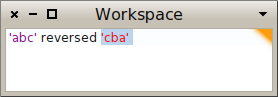
\includegraphics[width={.6}\textwidth]{workspace}
% \end{center}

\subsection{The Pharo Code Browser}

The Pharo code browser is composed of 5 panes:

\begin{itemize}
\item The \emph{packages} pane shows all the packages of the system.
\item The \emph{classes} pane shows the class hierarchy of the
  selected package; the \emph{class side} checkbox allows for getting
  the methods of the metaclass.
\item The \emph{protocols} pane groups the methods of the selected
  class to ease navigation.  When a protocol name starts with a \emph{*}, methods of this
  protocol belong to a different package (\eg the \emph{*Fuel}
  protocol groups methods that belong to the \emph{Fuel} package);
\item The \emph{methods} pane lists the methods of the selected
  protocol; icons are clickable and trigger special actions;
\item The \emph{source code} pane shows the source code of the
  selected method. 
\end{itemize}

\begin{center}
  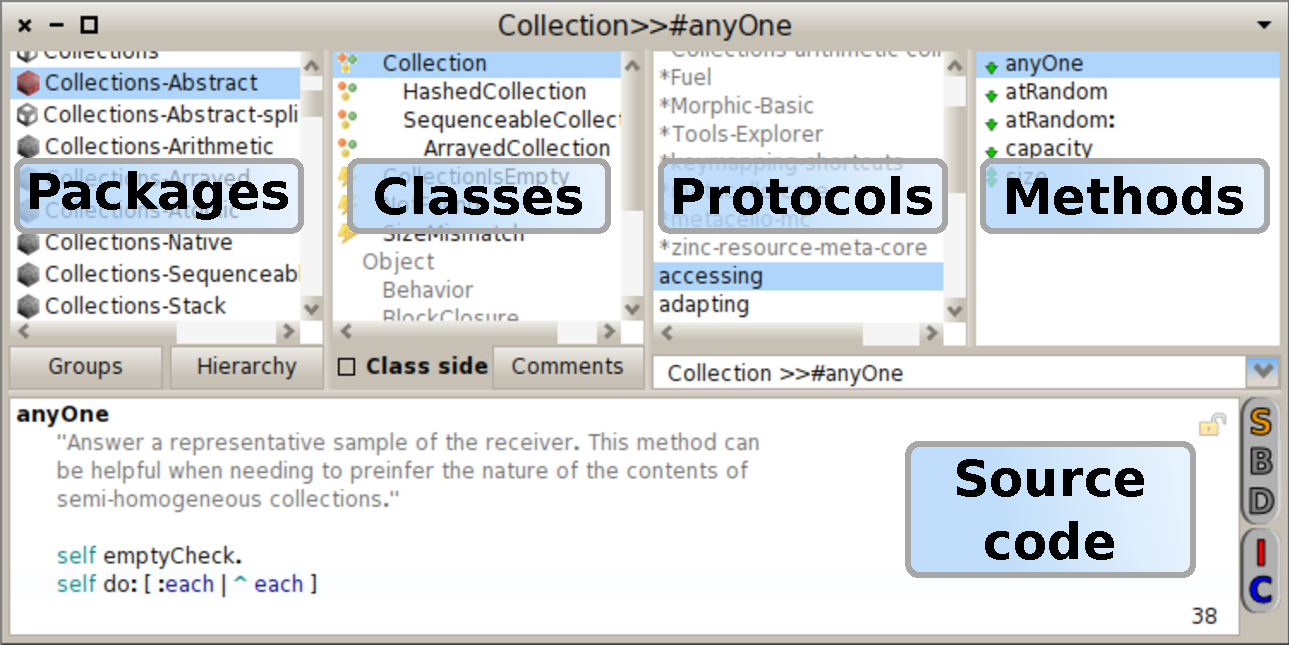
\includegraphics[width=\textwidth]{nautilus-anotated}
\end{center}

To add a package: first column + menu add package

\subsection{Defining a class}
To add a class, edit the proposed template!
The following expression defines the class \code{Counter} as a subclass of \code{Object}.
It defines two instance variables \code{count} and \code{initialValue} inside the package \code{MyCounter}.

\begin{displaycode}
Object subclass: #Counter
   instanceVariableNames: 'count initialValue'
   classVariableNames: '' 
   package: 'MyCounter'
\end{displaycode}

The method \code{initialize} is automatically invoked when a new instance is created by sending the message \code{new} to the class i.e.,\code{Counter new}. 

\begin{displaycode}
initialize 
    super initialize.
    count := 0. 
\end{displaycode}


%\pagebreak{}

%\vspace*{\fill}


\subsection{Unit testing}
 A test must be implemented in a method whose name has a \code{test} prefix and in a class that
subclasses \code{TestCase}.

\begin{displaycode}
\textcolor{darkBlue}{OrderedCollectionTest}\,>>\,testAdd
  | \textcolor{darkBlue}{added} |
  \textcolor{darkBlue}{added} := \textcolor{darkBlue}{collection} add: \textcolor{string}{'foo'}.
  \textcolor{darkCyan}{self} assert: \textcolor{darkBlue}{added} == \textcolor{string}{'foo'}.
  \textcolor{darkCyan}{self} assert: (\textcolor{darkBlue}{collection} includes: \textcolor{string}{'foo'}).
\end{displaycode}

The \code{\textcolor{darkBlue}{OrderedCollectionTest}\,>{}>\,testAdd}
notation indicates that the following text is the content of the
method \code{\textbf{testAdd}} in the class
\code{\textcolor{darkBlue}{OrderedCollectionTest}}. The second line
declares the variable \code{\textcolor{darkBlue}{added}}. To execute
unit-tests, open the \code{Test Runner} tool.



\section{A simple, uniform and powerful model}

Pharo has a simple dynamically-typed object model:

\begin{itemize}
\item everything is an object --- instance of a class;
\item classes are objects too;
\item there is single inheritance between classes;
\item traits are groups of methods that can be reused orthogonally to inheritance;
\item instance variables are protected;
\item methods are public and virtual;
\item blocks are lexical closures a.k.a. anonymous methods;
\item computation happens only via message sends (and variable assignment).
\end{itemize}

\textbf{Less is more:} There is no type declaration, no primitive
objects, no generic types, no modifiers, no operators, no inner
classes, no constructor, and no static methods. You will never need them in
Pharo!







\vfill{}

\end{document}

%%% Local Variables:
%%% mode: latex
%%% TeX-master: t
%%% End:
